\documentclass[conference]{IEEEtran}
\usepackage[utf8]{inputenc}
\usepackage{graphicx}
\usepackage{hyperref}
\usepackage{listings}
\usepackage{xcolor}
\usepackage{float}
\usepackage{amsmath}
\usepackage{booktabs}

\definecolor{codegreen}{rgb}{0,0.6,0}
\definecolor{codegray}{rgb}{0.5,0.5,0.5}
\definecolor{codepurple}{rgb}{0.58,0,0.82}
\definecolor{backcolour}{rgb}{0.95,0.95,0.92}

\lstdefinestyle{mystyle}{
    backgroundcolor=\color{backcolour},
    commentstyle=\color{codegreen},
    keywordstyle=\color{codepurple},
    numberstyle=\tiny\color{codegray},
    basicstyle=\ttfamily\scriptsize,
    breaklines=true,
    frame=single,
}
\lstset{style=mystyle}

\title{Accessible Public Transit Trip Planner:\\A Cloud-Native Application Using AWS Services}
\author{
\IEEEauthorblockN{Rakesh Kunchala}
\IEEEauthorblockA{Student ID: x25176862\\
x25176862@student.ncirl.ie\\
National College of Ireland\\
Cloud Platform Programming}
}

\begin{document}

\maketitle

\begin{abstract}
This paper presents the design, implementation, and evaluation of an Accessible Public Transit Trip Planner built as a cloud-native application leveraging seven Amazon Web Services (AWS). The system provides route planning, accessibility scoring, fare estimation, and schedule management through a Flask REST API backend, a React frontend, and a custom object-oriented Python library called \texttt{transitplan}. The application implements full CRUD operations for transit entities and integrates Amazon RDS, S3, Location Service, SQS, Secrets Manager, CloudFront, and Comprehend. All services operate in local mock mode for development and testing, with seamless production deployment capability. The system demonstrates practical cloud platform programming patterns including the application factory pattern, service abstraction layers, and comprehensive automated testing with 105 passing tests.
\end{abstract}

\begin{IEEEkeywords}
cloud computing, AWS, transit planning, accessibility, REST API, microservices
\end{IEEEkeywords}

\section{Introduction}

Public transit accessibility remains a significant challenge in urban areas. Many trip planning applications fail to account for the diverse needs of passengers with disabilities, including wheelchair users, visually impaired travelers, and hearing-impaired commuters. This project addresses these gaps by developing a comprehensive, cloud-native transit trip planner that places accessibility at its core.

The application integrates seven AWS services to provide a scalable, maintainable solution. A custom Python library, \texttt{transitplan}, encapsulates the domain logic using object-oriented programming principles, including route modeling, shortest-path algorithms, accessibility scoring, fare calculation, and schedule management.

The primary contributions of this work are: (1) a custom OOP library for accessible transit planning with Dijkstra-based routing, (2) integration of seven AWS services with local mock modes enabling offline development, (3) full CRUD REST API with 35 integration tests, and (4) a React frontend providing an intuitive user experience for trip planning and accessibility analysis.

\section{System Architecture}

The system follows a three-tier architecture comprising a React frontend, Flask REST API backend, and cloud service layer. Figure~\ref{fig:architecture} illustrates the overall system architecture.

\begin{figure}[H]
\centering
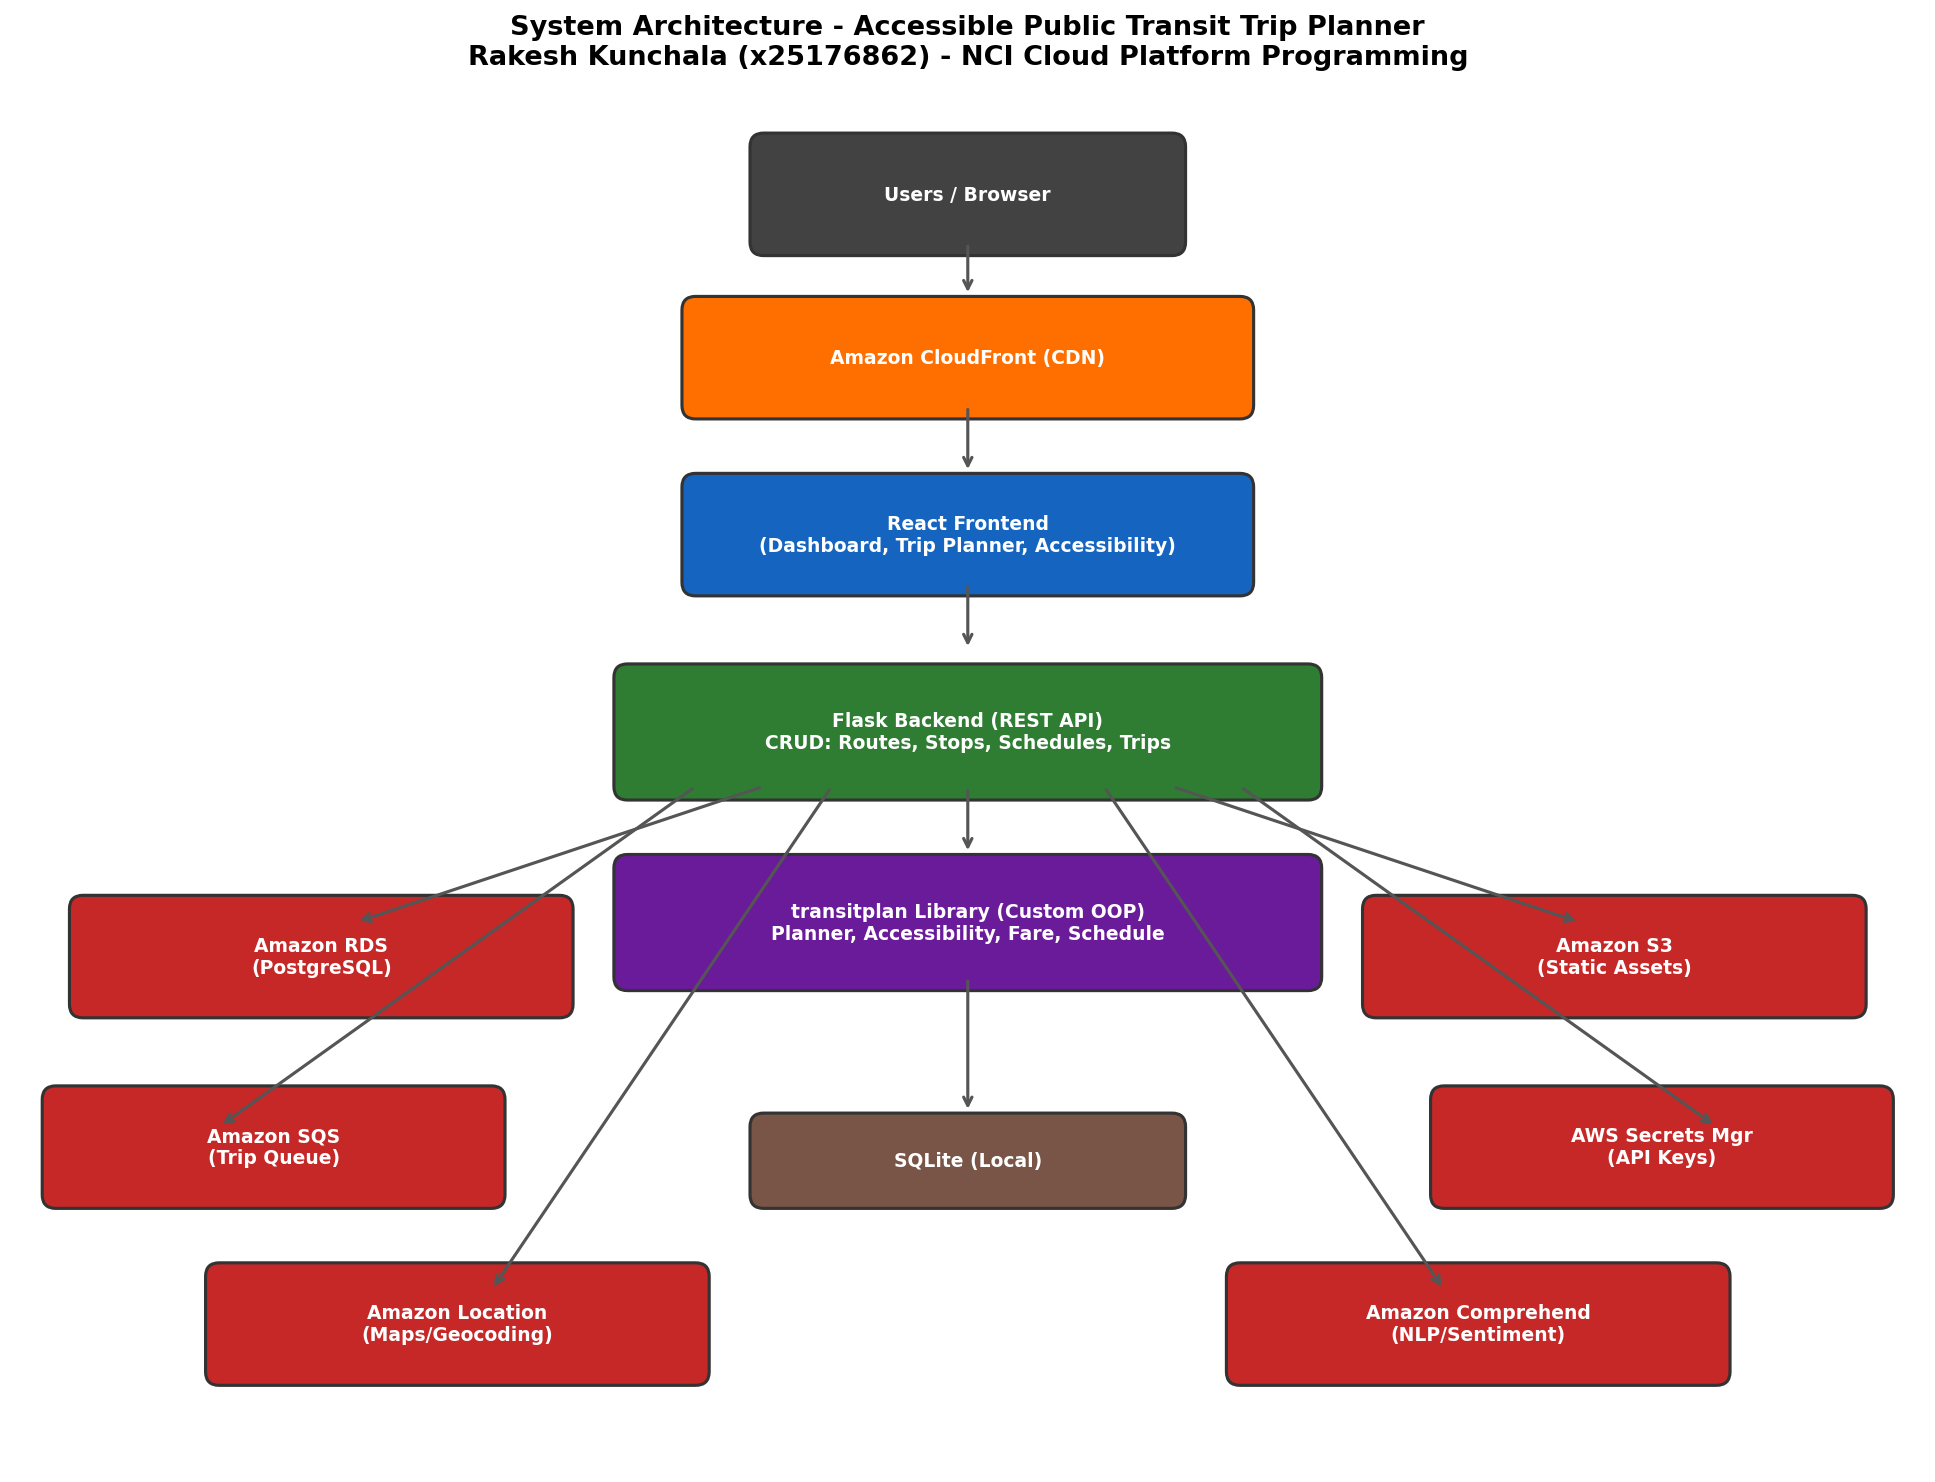
\includegraphics[width=\columnwidth]{architecture_diagram.png}
\caption{System architecture showing the three-tier design with seven AWS service integrations.}
\label{fig:architecture}
\end{figure}

\subsection{Frontend Layer}

The React frontend provides seven pages: Dashboard, Routes, Stops, Schedules, Trip Planner, Accessibility, and AWS Status. It communicates with the backend via REST API calls and is distributed through Amazon CloudFront for production deployments.

\subsection{Backend Layer}

The Flask backend implements the application factory pattern, enabling multiple configurations (development, testing, production). It exposes RESTful CRUD endpoints for routes, stops, schedules, and trips, plus AWS service endpoints for geocoding, sentiment analysis, and queue management.

\subsection{Custom Library Layer}

The \texttt{transitplan} library provides five modules: \texttt{models.py} for core data structures, \texttt{planner.py} for trip planning algorithms, \texttt{accessibility.py} for scoring, \texttt{fare.py} for fare estimation, and \texttt{schedule\_calc.py} for time calculations.

\section{AWS Service Integration}

Seven AWS services are integrated, each with a dedicated service wrapper class that supports both production and local mock modes.

\subsection{Amazon RDS (PostgreSQL)}

Amazon RDS hosts the PostgreSQL database storing routes, stops, schedules, trips, and accessibility features. SQLAlchemy ORM provides database abstraction, with SQLite used locally and PostgreSQL in production.

\subsection{Amazon S3}

Amazon S3 stores static assets including map tiles, route data exports, and uploaded media. The \texttt{S3Service} class provides upload, download, delete, and list operations with an in-memory mock store for development.

\subsection{Amazon Location Service}

The Location Service provides geocoding (address to coordinates) and reverse geocoding capabilities. Mock mode uses a dictionary of Dublin transit station coordinates for testing.

\subsection{Amazon SQS}

SQS manages asynchronous trip planning requests. When users submit complex route queries, they are enqueued for processing. The mock implementation uses Python's \texttt{deque} for in-memory queue simulation.

\subsection{AWS Secrets Manager}

Secrets Manager securely stores database credentials, API keys, and JWT secrets. The mock mode uses an in-memory dictionary, while production retrieves secrets via the AWS SDK.

\subsection{Amazon CloudFront}

CloudFront serves as the CDN for the React frontend, providing low-latency global distribution. The service wrapper manages cache invalidation and distribution URL generation.

\subsection{Amazon Comprehend}

Comprehend analyzes user feedback and reviews for sentiment (positive, negative, neutral, mixed) and extracts key phrases. The mock mode uses keyword-matching for sentiment classification.

\section{Custom Library: transitplan}

\subsection{Data Models}

The library defines five core classes: \texttt{Stop} (location with accessibility attributes), \texttt{Route} (ordered stop sequence), \texttt{Schedule} (departure/arrival times), \texttt{Connection} (directed edge between stops), and \texttt{TransitNetwork} (graph container with adjacency lists).

\subsection{Trip Planning Algorithm}

The \texttt{TripPlanner} class implements two strategies. The ``shortest'' strategy uses Dijkstra's algorithm with travel time as edge weight. The ``fewest transfers'' strategy adds a heavy penalty (50 minutes) for route changes, effectively minimizing transfers.

\begin{lstlisting}[language=Python, caption=Trip planning with Dijkstra's algorithm]
def _plan_shortest(self, origin_id, dest_id):
    dist = {origin_id: 0.0}
    prev = {origin_id: None}
    pq = [(0.0, origin_id)]
    visited = set()
    while pq:
        cost, current = heapq.heappop(pq)
        if current in visited: continue
        visited.add(current)
        if current == dest_id: break
        for conn in self.network.get_neighbors(current):
            next_id = conn.to_stop.stop_id
            new_cost = cost + conn.travel_minutes
            if next_id not in dist or new_cost < dist[next_id]:
                dist[next_id] = new_cost
                prev[next_id] = (current, conn)
                heapq.heappush(pq, (new_cost, next_id))
    return self._reconstruct_trip(origin_id, dest_id, prev)
\end{lstlisting}

\subsection{Accessibility Scoring}

The \texttt{AccessibilityScorer} evaluates stops using weighted criteria: wheelchair access (40\%), audio announcements (25\%), visual displays (20\%), and tactile paving (15\%). Route scores average across stops; trip scores use the minimum (weakest link).

\subsection{Fare Estimation}

The \texttt{FareCalculator} supports three models: flat rate, zone-based, and distance-based. It applies transfer discounts (25\%) and concession discounts (50\%), clamped between minimum and maximum fare limits.

\section{CRUD Operations}

The application provides full Create, Read, Update, Delete operations for four entities through RESTful endpoints:

\begin{table}[H]
\centering
\caption{CRUD API Endpoints}
\begin{tabular}{@{}llll@{}}
\toprule
Entity & Create & Read & Update/Delete \\
\midrule
Routes & POST /api/routes & GET /api/routes & PUT/DELETE /api/routes/\{id\} \\
Stops & POST /api/stops & GET /api/stops & PUT/DELETE /api/stops/\{id\} \\
Schedules & POST /api/schedules & GET /api/schedules & PUT/DELETE /api/schedules/\{id\} \\
Trips & POST /api/trips & GET /api/trips & PUT/DELETE /api/trips/\{id\} \\
\bottomrule
\end{tabular}
\end{table}

Each endpoint validates input, handles duplicates with 409 responses, and returns appropriate HTTP status codes. The implementation uses SQLAlchemy models with Flask-SQLAlchemy for database operations.

\section{Component Architecture}

Figure~\ref{fig:components} shows the detailed component relationships across the system layers.

\begin{figure}[H]
\centering
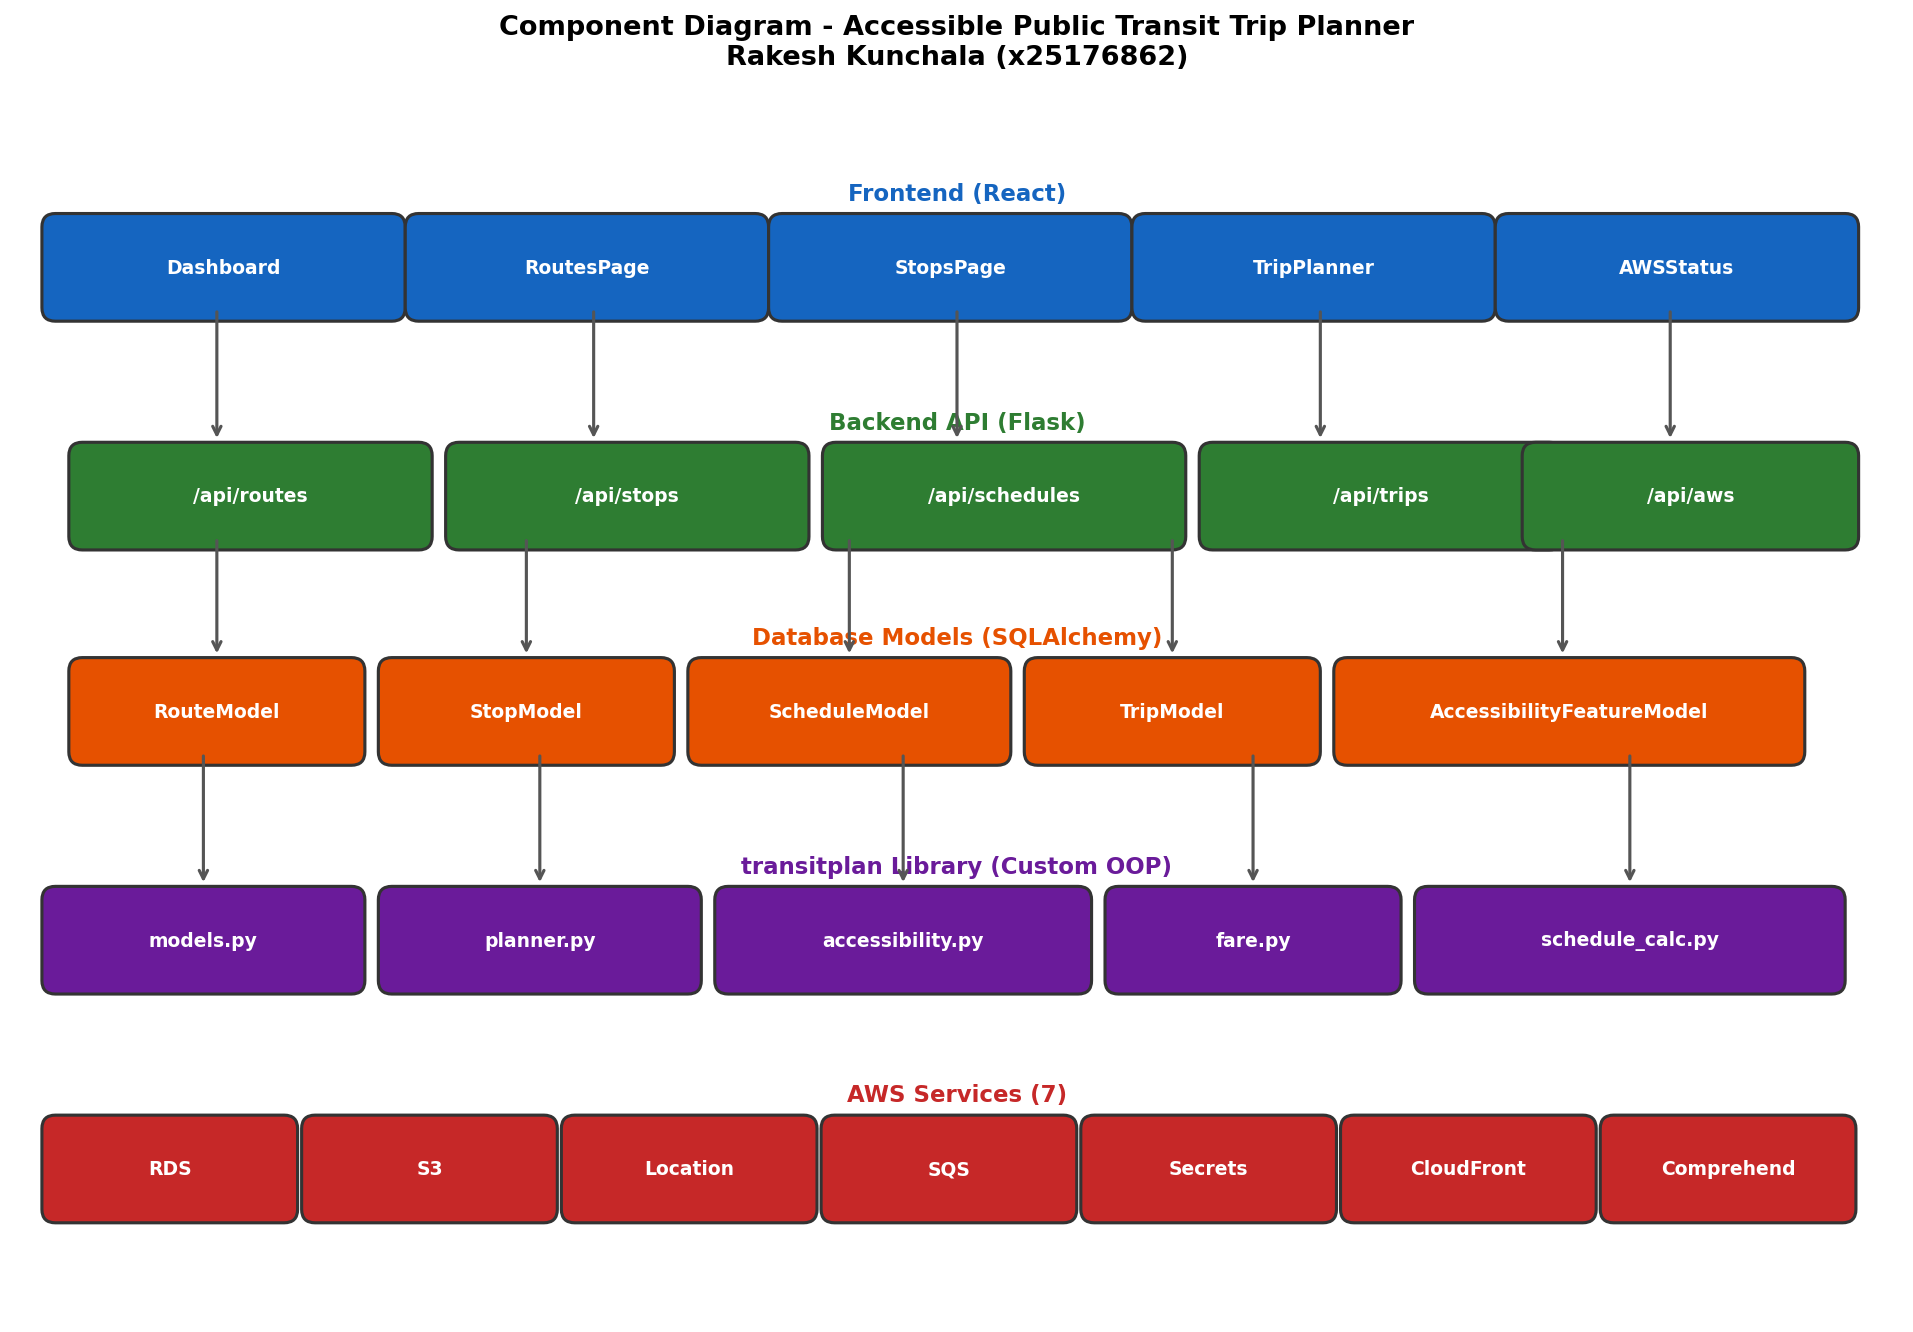
\includegraphics[width=\columnwidth]{component_diagram.png}
\caption{Component diagram showing module relationships across frontend, backend, models, library, and AWS service layers.}
\label{fig:components}
\end{figure}

\section{Testing}

The project includes comprehensive automated testing at two levels:

\textbf{Unit Tests (70 tests):} The \texttt{transitplan} library has tests covering models (17 tests), trip planner (10 tests), accessibility scoring (14 tests), fare calculation (12 tests), and schedule calculations (14 tests). The remaining 3 tests come from edge cases.

\textbf{Integration Tests (35 tests):} The Flask API tests cover CRUD operations for routes (8 tests), stops (7 tests), schedules (5 tests), and trips (5 tests), plus AWS service endpoint tests (10 tests).

All 105 tests pass successfully, achieving comprehensive coverage of the application logic and API endpoints.

\section{Deployment Considerations}

The application is designed for AWS deployment with the following configuration:
The database tier uses Amazon RDS PostgreSQL (db.t3.micro for development), while the backend is deployed on AWS Elastic Beanstalk or ECS Fargate. The frontend is served through S3 static hosting with a CloudFront distribution for global content delivery. Credentials are managed through AWS Secrets Manager with support for credential rotation, and asynchronous trip planning requests are handled via an SQS Standard Queue.

All services use local mock mode during development, toggled via the \texttt{USE\_LOCAL\_MOCKS} environment variable.

\section{Conclusion}

This project demonstrates a practical cloud-native application integrating seven AWS services for accessible public transit planning. The custom \texttt{transitplan} library provides reusable, well-tested OOP components for route modeling, trip planning with Dijkstra's algorithm, accessibility scoring, and fare estimation. The application achieves full CRUD functionality with comprehensive test coverage (105 tests), a responsive React frontend, and a clean separation of concerns through the service abstraction pattern. Future work could extend the system with real-time transit data feeds, machine learning-based demand prediction, and expanded accessibility features including route-specific audio navigation.

\begin{thebibliography}{00}
\bibitem{b1} Amazon Web Services, ``AWS Documentation,'' \url{https://docs.aws.amazon.com/}, 2024.
\bibitem{b2} M. Grinberg, ``Flask Web Development,'' O'Reilly Media, 2nd ed., 2018.
\bibitem{b3} T. H. Cormen et al., ``Introduction to Algorithms,'' MIT Press, 4th ed., 2022.
\bibitem{b4} W3C, ``Web Content Accessibility Guidelines (WCAG) 2.1,'' \url{https://www.w3.org/TR/WCAG21/}, 2018.
\bibitem{b5} React Documentation, ``React: A JavaScript Library for Building User Interfaces,'' \url{https://react.dev/}, 2024.
\bibitem{b6} SQLAlchemy Documentation, ``SQLAlchemy ORM Tutorial,'' \url{https://docs.sqlalchemy.org/}, 2024.
\bibitem{b7} E. W. Dijkstra, ``A Note on Two Problems in Connexion with Graphs,'' Numerische Mathematik, vol. 1, pp. 269--271, 1959.
\bibitem{b8} Transport for Ireland, ``National Transport Authority Open Data,'' \url{https://www.transportforireland.ie/}, 2024.
\end{thebibliography}

\end{document}
